%%%%%%%%%%%%%%%%%%%%%%%%%%%%%%%%%%%%%%%%%
% Lachaise Assignment
% LaTeX Template
% Version 1.0 (26/6/2018)
%
% This template originates from:
% http://www.LaTeXTemplates.com
%
% Authors:
% Marion Lachaise & François Févotte
% Vel (vel@LaTeXTemplates.com)
%
% License:
% CC BY-NC-SA 3.0 (http://creativecommons.org/licenses/by-nc-sa/3.0/)
% 
%%%%%%%%%%%%%%%%%%%%%%%%%%%%%%%%%%%%%%%%%

%----------------------------------------------------------------------------------------
%	PACKAGES AND OTHER DOCUMENT CONFIGURATIONS

%----------------------------------------------------------------------------------------

\documentclass{article}

\usepackage{graphicx} 
\usepackage{subfigure}

%%%%%%%%%%%%%%%%%%%%%%%%%%%%%%%%%%%%%%%%%
% Lachaise Assignment
% Structure Specification File
% Version 1.0 (26/6/2018)
%
% This template originates from:
% http://www.LaTeXTemplates.com
%
% Authors:
% Marion Lachaise & François Févotte
% Vel (vel@LaTeXTemplates.com)
%
% License:
% CC BY-NC-SA 3.0 (http://creativecommons.org/licenses/by-nc-sa/3.0/)
% 
%%%%%%%%%%%%%%%%%%%%%%%%%%%%%%%%%%%%%%%%%

%----------------------------------------------------------------------------------------
%	PACKAGES AND OTHER DOCUMENT CONFIGURATIONS
%----------------------------------------------------------------------------------------

\usepackage{amsmath,amsfonts,stmaryrd,amssymb} % Math packages

\usepackage{enumerate} % Custom item numbers for enumerations

\usepackage[ruled]{algorithm2e} % Algorithms

\usepackage[framemethod=tikz]{mdframed} % Allows defining custom boxed/framed environments

\usepackage{listings} % File listings, with syntax highlighting
\lstset{
	basicstyle=\ttfamily, % Typeset listings in monospace font
}

%----------------------------------------------------------------------------------------
%	DOCUMENT MARGINS
%----------------------------------------------------------------------------------------

\usepackage{geometry} % Required for adjusting page dimensions and margins

\geometry{
	paper=a4paper, % Paper size, change to letterpaper for US letter size
	top=2.5cm, % Top margin
	bottom=3cm, % Bottom margin
	left=2.5cm, % Left margin
	right=2.5cm, % Right margin
	headheight=14pt, % Header height
	footskip=1.5cm, % Space from the bottom margin to the baseline of the footer
	headsep=1.2cm, % Space from the top margin to the baseline of the header
	%showframe, % Uncomment to show how the type block is set on the page
}

%----------------------------------------------------------------------------------------
%	FONTS
%----------------------------------------------------------------------------------------

\usepackage[utf8]{inputenc} % Required for inputting international characters
\usepackage[T1]{fontenc} % Output font encoding for international characters

\usepackage{XCharter} % Use the XCharter fonts

%----------------------------------------------------------------------------------------
%	COMMAND LINE ENVIRONMENT
%----------------------------------------------------------------------------------------

% Usage:
% \begin{commandline}
%	\begin{verbatim}
%		$ ls
%		
%		Applications	Desktop	...
%	\end{verbatim}
% \end{commandline}

\mdfdefinestyle{commandline}{
	leftmargin=10pt,
	rightmargin=10pt,
	innerleftmargin=15pt,
	middlelinecolor=black!50!white,
	middlelinewidth=2pt,
	frametitlerule=false,
	backgroundcolor=black!5!white,
	frametitle={Command Line},
	frametitlefont={\normalfont\sffamily\color{white}\hspace{-1em}},
	frametitlebackgroundcolor=black!50!white,
	nobreak,
}

% Define a custom environment for command-line snapshots
\newenvironment{commandline}{
	\medskip
	\begin{mdframed}[style=commandline]
}{
	\end{mdframed}
	\medskip
}

%----------------------------------------------------------------------------------------
%	FILE CONTENTS ENVIRONMENT
%----------------------------------------------------------------------------------------

% Usage:
% \begin{file}[optional filename, defaults to "File"]
%	File contents, for example, with a listings environment
% \end{file}

\mdfdefinestyle{file}{
	innertopmargin=1.6\baselineskip,
	innerbottommargin=0.8\baselineskip,
	topline=false, bottomline=false,
	leftline=false, rightline=false,
	leftmargin=2cm,
	rightmargin=2cm,
	singleextra={%
		\draw[fill=black!10!white](P)++(0,-1.2em)rectangle(P-|O);
		\node[anchor=north west]
		at(P-|O){\ttfamily\mdfilename};
		%
		\def\l{3em}
		\draw(O-|P)++(-\l,0)--++(\l,\l)--(P)--(P-|O)--(O)--cycle;
		\draw(O-|P)++(-\l,0)--++(0,\l)--++(\l,0);
	},
	nobreak,
}

% Define a custom environment for file contents
\newenvironment{file}[1][File]{ % Set the default filename to "File"
	\medskip
	\newcommand{\mdfilename}{#1}
	\begin{mdframed}[style=file]
}{
	\end{mdframed}
	\medskip
}

%----------------------------------------------------------------------------------------
%	NUMBERED QUESTIONS ENVIRONMENT
%----------------------------------------------------------------------------------------

% Usage:
% \begin{question}[optional title]
%	Question contents
% \end{question}

\mdfdefinestyle{question}{
	innertopmargin=1.2\baselineskip,
	innerbottommargin=0.8\baselineskip,
	roundcorner=5pt,
	nobreak,
	singleextra={%
		\draw(P-|O)node[xshift=1em,anchor=west,fill=white,draw,rounded corners=5pt]{%
		Question \theQuestion\questionTitle};
	},
}

\newcounter{Question} % Stores the current question number that gets iterated with each new question

% Define a custom environment for numbered questions
\newenvironment{question}[1][\unskip]{
	\bigskip
	\stepcounter{Question}
	\newcommand{\questionTitle}{~#1}
	\begin{mdframed}[style=question]
}{
	\end{mdframed}
	\medskip
}

%----------------------------------------------------------------------------------------
%	WARNING TEXT ENVIRONMENT
%----------------------------------------------------------------------------------------

% Usage:
% \begin{warn}[optional title, defaults to "Warning:"]
%	Contents
% \end{warn}

\mdfdefinestyle{warning}{
	topline=false, bottomline=false,
	leftline=false, rightline=false,
	nobreak,
	singleextra={%
		\draw(P-|O)++(-0.5em,0)node(tmp1){};
		\draw(P-|O)++(0.5em,0)node(tmp2){};
		\fill[black,rotate around={45:(P-|O)}](tmp1)rectangle(tmp2);
		\node at(P-|O){\color{white}\scriptsize\bf !};
		\draw[very thick](P-|O)++(0,-1em)--(O);%--(O-|P);
	}
}

% Define a custom environment for warning text
\newenvironment{warn}[1][Warning:]{ % Set the default warning to "Warning:"
	\medskip
	\begin{mdframed}[style=warning]
		\noindent{\textbf{#1}}
}{
	\end{mdframed}
}

%----------------------------------------------------------------------------------------
%	INFORMATION ENVIRONMENT
%----------------------------------------------------------------------------------------

% Usage:
% \begin{info}[optional title, defaults to "Info:"]
% 	contents
% 	\end{info}

\mdfdefinestyle{info}{%
	topline=false, bottomline=false,
	leftline=false, rightline=false,
	nobreak,
	singleextra={%
		\fill[black](P-|O)circle[radius=0.4em];
		\node at(P-|O){\color{white}\scriptsize\bf i};
		\draw[very thick](P-|O)++(0,-0.8em)--(O);%--(O-|P);
	}
}

% Define a custom environment for information
\newenvironment{info}[1][Info:]{ % Set the default title to "Info:"
	\medskip
	\begin{mdframed}[style=info]
		\noindent{\textbf{#1}}
}{
	\end{mdframed}
}
 % Include the file specifying the document structure and custom commands

%----------------------------------------------------------------------------------------
%	ASSIGNMENT INFORMATION
%----------------------------------------------------------------------------------------

\title{CMPT742: Assignment \#1} % Title of the assignment

\author{Lin Duan 301369502 \& Jingwen Zhang\\ \texttt{duanlind@sfu.ca \& jingwen\_zhang\_2\@sfu.ca}} % Author name and email address

\date{Simon Fraser University--- \today} % University, school and/or department name(s) and a date

%----------------------------------------------------------------------------------------

\begin{document}

\maketitle % Print the title

%----------------------------------------------------------------------------------------
%	INTRODUCTION
%----------------------------------------------------------------------------------------

\section*{Introducation} % Unnumbered section

In this assignment we use AlexNet and Resnet18 as the training model to detect the facial landmark. And in this report, we will first describe the network struture and the training process (data augmentation, learning rate parameters…). Then we will show the training/validation loss curve from both Alexnet and Resnet18. Finally, we will show the test result from both.


\section{Network Structure} % Numbered section



%------------------------------------------------

\subsection{Alexnet Structure}

The Alexnet structure adapts to this project would be:

\begin{center} 
	\begin{tabular}{ | l | l |} 
		\hline 
		Layer Name & Tensor Size      \\ \hline 
		iuput image & 227$\times$227$\times$3   \\ \hline 
		Conv\-1 & 55$\times$55$\times$96   \\ \hline 
		Maxpool-1 & 27$\times$27$\times$96   \\ \hline 
		Conv\-2 & 27$\times$27$\times$256   \\ \hline 
		Maxpool-2 & 13$\times$13$\times$256   \\ \hline 
		Conv\-3 & 13$\times$13$\times$384   \\ \hline 
		Conv\-4 & 13$\times$13$\times$384   \\ \hline 
		Conv\-5 & 13$\times$13$\times$256   \\ \hline 
		Maxpool-3 & 6$\times$6$\times$256   \\ \hline
		FC\-1 & 512  \\ \hline
		FC\-2 & 256  \\ \hline
		FC\-3 & 7$\times$2  \\ \hline
		Output & 14  \\ \hline

	\end{tabular}  
\end{center} 



\begin{commandline}
	\begin{verbatim}
net = models.alexnet(pretrained=pretrained)
net.classifier = nn.Sequential(
nn.Dropout(),
nn.Linear(256 * 6 * 6, 512),
nn.ReLU(inplace=True),
nn.Dropout(),
nn.Linear(512, 256),
nn.ReLU(inplace=True),
nn.Linear(256, 14),
)
net.cuda()
	\end{verbatim}
\end{commandline}






\subsection{Resnet Structure}

We use Resnet18 as our training model. The Resnet18 structure adapts to this project would be:

\begin{center} 
	\begin{tabular}{ | l | l | l |} 
		\hline 
		Layer Name & Tensor Size      & 18\-layer  \\ \hline 
		conv1  & 112$\times$112 & 7$\times$7,stride 2  \\ \hline 
		&                         & 3$\times$3 max pool,stride 2  \\ \hline 
		conv2\_ x    &  56$\times$56  & \( \left [  \begin{array}{lcl}  3 \times 3, 64 \\   3 \times 3, 64    \end{array}   \right] \times 2 \)\\ \hline
		conv3\_ x    &  28$\times$28  & \( \left [  \begin{array}{lcl}  3 \times 3, 128\\   3 \times 3, 128   \end{array}   \right] \times 2 \)\\ \hline
		conv4\_ x    &  14$\times$14  & \( \left [  \begin{array}{lcl}  3 \times 3, 256\\   3 \times 3, 256   \end{array}   \right] \times 2 \)\\ \hline
		conv5\_ x    &  7$\times$7     & \( \left [  \begin{array}{lcl}  3 \times 3, 512\\   3 \times 3, 512 \end{array}   \right] \times 2 \)\\ \hline
		& 1$\times 1$     & average pool, 14\-d fc, softmax \\ \hline
	\end{tabular}  
\end{center} 

\begin{file}[resnet\_train.py]
	\begin{lstlisting}[language=Python]
	#! /usr/bin/python3
	import resnet
	\end{lstlisting}
\end{file}

And part of the commond line for Resnet18 would be:
\begin{commandline}
	\begin{verbatim}
def resnet18(pretrained=False, **kwargs):
"""Constructs a ResNet-18 model.

Args:
pretrained (bool): If True, returns a model pre-trained on ImageNet
"""
model = ResNet(BasicBlock, [2, 2, 2, 2], **kwargs)
if pretrained:
# model.load_state_dict(model_zoo.load_url(model_urls['resnet18']))
pretrained_dict = model_zoo.load_url(model_urls['resnet18'])
model_dict = model.state_dict()
# 1. filter out unnecessary keys
pretrained_dict = {k: v for k, v in pretrained_dict.items() if k in model_dict 
... : and v.size() ==model_dict[k].size()}
# 2. overwrite entries in the existing state dict
model_dict.update(pretrained_dict) 
# 3. load the new state dict
model.load_state_dict(model_dict)
return model
	\end{verbatim}
\end{commandline}

\section{Training Process}
\subsection{Data Augumentation}
In order to prevent overfitting, we implement augmentation on images in two ways: Random Cropping and Random Flipping.

Random cropping means to manipulate the bonuding box by adding random offset.

\begin{commandline}
	\begin{verbatim}
	 # random crop
	if 'rcrop' in self.transform:
	if random.random() < 0.5:
	top = np.random.randint(0, int(landmarks[:,0].min() - bbox[0][0])+1) - random_crop_r
	left = np.random.randint(0, int(landmarks[:,1].min() - bbox[0][1])+1) - random_crop_r
	offset = [[top,left],[top,left]]
	bbox += offset
	img = img.crop((bbox[0][0], bbox[0][1], bbox[1][0], bbox[1][1]))
	img = img.resize((img_size, img_size))
	landmarks_ = []
	for coor in landmarks:
	coor = coor - bbox[0]
	coor[0] = coor[0] / w  # 0~225
	coor[1] = coor[1] / h 
	landmarks_.append(coor)
	landmarks_ = np.array(landmarks_, dtype=np.float).T
	

	\end{verbatim}
\end{commandline}


Random filpping means to flip the image horizontally. 

\begin{commandline}
	\begin{verbatim}
	# random flip
	if 'flip' in self.transform:
	if random.random() < 0.5:
	img = img.transpose(Image.FLIP_LEFT_RIGHT)
	landmarks_[0] = np.ones(7) - landmarks_[0]
	
	img = np.array(img, dtype=np.float) / 255.0 * 2 - 1
	img_tensor = torch.from_numpy(img).float()
	landmarks_tensor = torch.from_numpy(landmarks_).float()
	\end{verbatim}
\end{commandline}

\subsection{Learning Parameters}
 We  choose 'Adam-Adaptive Moment Estimation' as optimizer. And we set learning rate to 0.0001.
 
 


	
%------------------------------------------------
\newpage
\section{Lossing Curve }

First, the lossing curve of Alexnet training is as following:

\begin{figure}[!h]
	\centering
	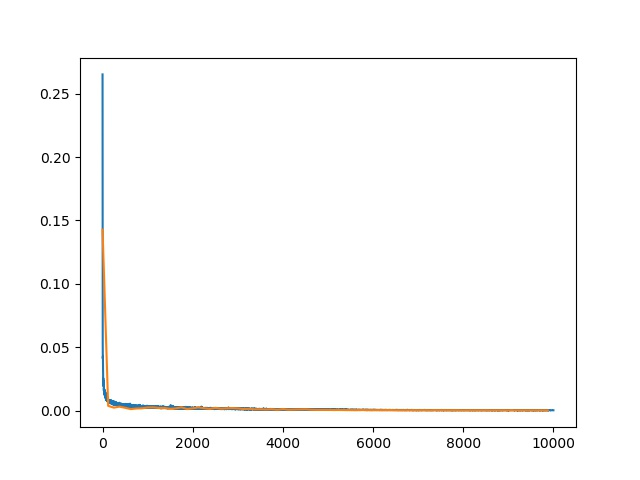
\includegraphics[width=3in]{alexloss}
	\caption{alexnet-lossing curve}
\end{figure}

The loss decline quickly in the first few iterations. 

Then, lossing curve of Resxnet training is as following:

\begin{figure}[!h]
	\centering
	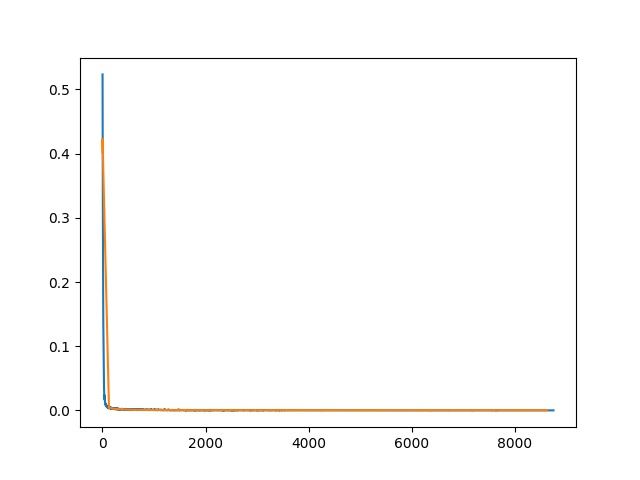
\includegraphics[width=3in]{resloss.jpg}
	\caption{resnet-lossing curve}
\end{figure}

\newpage
\section{Result and Accuracy}

We can see the test result and accuracy from Alexnet as below:(run for 80 epoches)

\begin{figure}[h]
	\begin{minipage}[t]{0.5\linewidth}
		\centering
		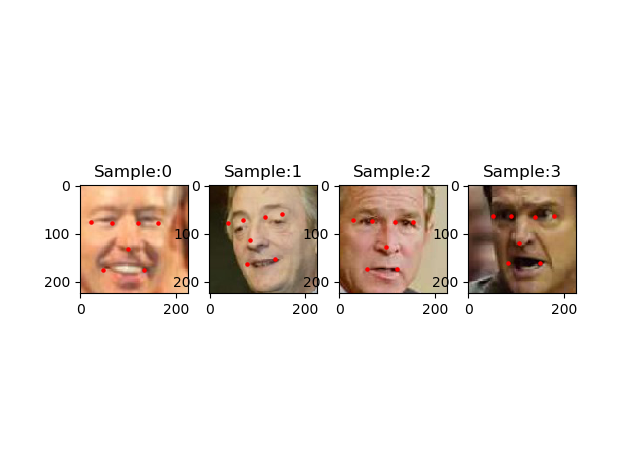
\includegraphics[width=2.5in]{alexresult.png}
		\caption{alex-result}
		\label{fig:side:a}
	\end{minipage}%
	\begin{minipage}[t]{0.5\linewidth}
		\centering
		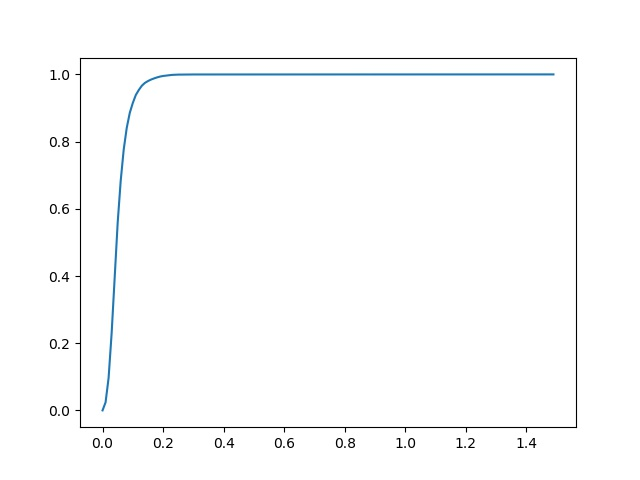
\includegraphics[width=2.5in]{alexradius.jpg}
		\caption{alex-accuracy}
		\label{fig:side:b}
	\end{minipage}
\end{figure}
 
 From the left image, we can see the test result is almost accurate with little deviation. The right image shows that within radius of and more than 0.2, nearly all test results are similar with original data.
 
The result and accuracy of Resnet :(run for 70 epoches)

\begin{figure}[h]
	\begin{minipage}[t]{0.5\linewidth}
		\centering
		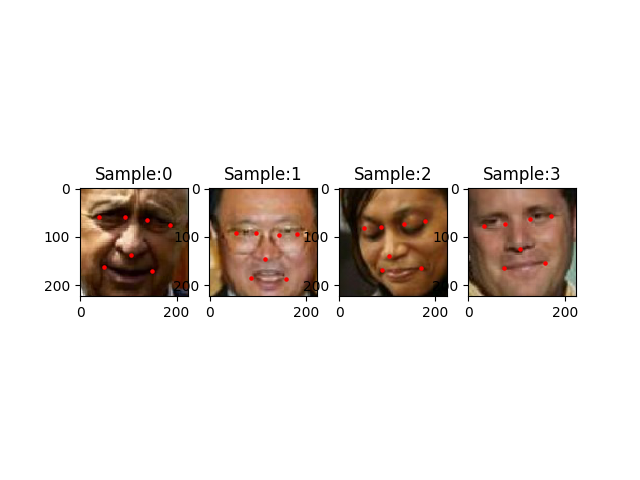
\includegraphics[width=2.5in]{resresult.png}
		\caption{res-result}
	\end{minipage}%
	\begin{minipage}[t]{0.5\linewidth}
		\centering
		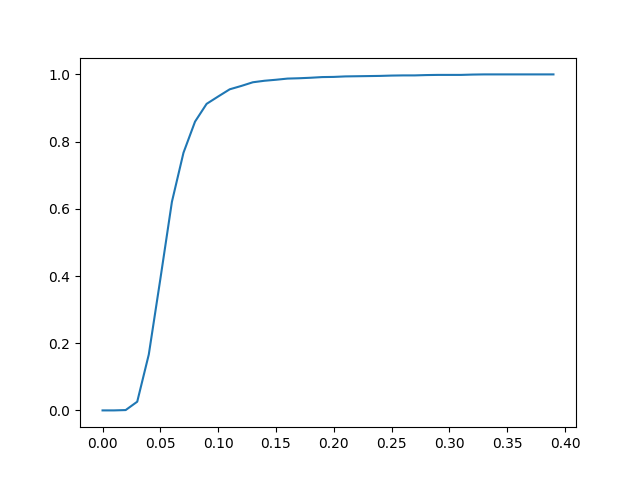
\includegraphics[width=2.5in]{resradius.png}
		\caption{res-accuracy}
	\end{minipage}
\end{figure}


% Warning text, with a custom title

%----------------------------------------------------------------------------------------

\end{document}
